% Decision tree / flowchart for Figure~\ref{fig:decision_tree}
% (Section 4: "Unified Methodology Framework").
%
% Revised version (Oct 2026), aligned with the case-study findings:
%  - Phase 1 declares the intended use (same instrument as in training, or
%    deployment on another instrument);
%  - Phase 2 checks whether the correlation structure of the declared input
%    uncertainty is stated, and otherwise bounds its random part from the data
%    (u_rand <= s) and splits u^2 = u_rand^2 + u_sys^2 (GUM 5.2.4, F.1.2.4);
%  - Phase 4 uses the paper's combination, Eqs. (combined_std_uncertainty) and
%    (model_uncertainty_decomposition), and propagates u_sys only for transfer;
%  - Phase 5 sends an LPU/MC discrepancy back to the input-uncertainty model
%    before Monte Carlo is adopted, and checks coverage at k = 1 and k = 2
%    in both directions (under- and over-coverage).
%
% Layout: two columns (Phases 1-3 left, Phases 4-5 right) so that the figure
% fits one page; validation returns use lettered connectors (A, B, C).
%
% Compiles with plain pdflatex (no standalone class needed) to a
% tightly-cropped vector PDF; copy decision_tree.pdf next to the paper .tex.
%
% Okabe-Ito colours, as in the case-study validation figures
% (make_validation_figure.py): blue = regression track, orange =
% classification track and decision nodes.
\documentclass{article}
\usepackage{amsmath}
\usepackage{amssymb}
\usepackage{tikz}
\usetikzlibrary{shapes.geometric, shapes.misc, arrows.meta, positioning, calc}

\definecolor{okBlue}{HTML}{0072B2}
\definecolor{okOrange}{HTML}{D55E00}

\pagestyle{empty}
\hyphenpenalty=10000
\exhyphenpenalty=10000
\newsavebox{\figbox}
\newlength{\figborder}
\setlength{\figborder}{4pt}

\begin{document}
\begin{lrbox}{\figbox}%
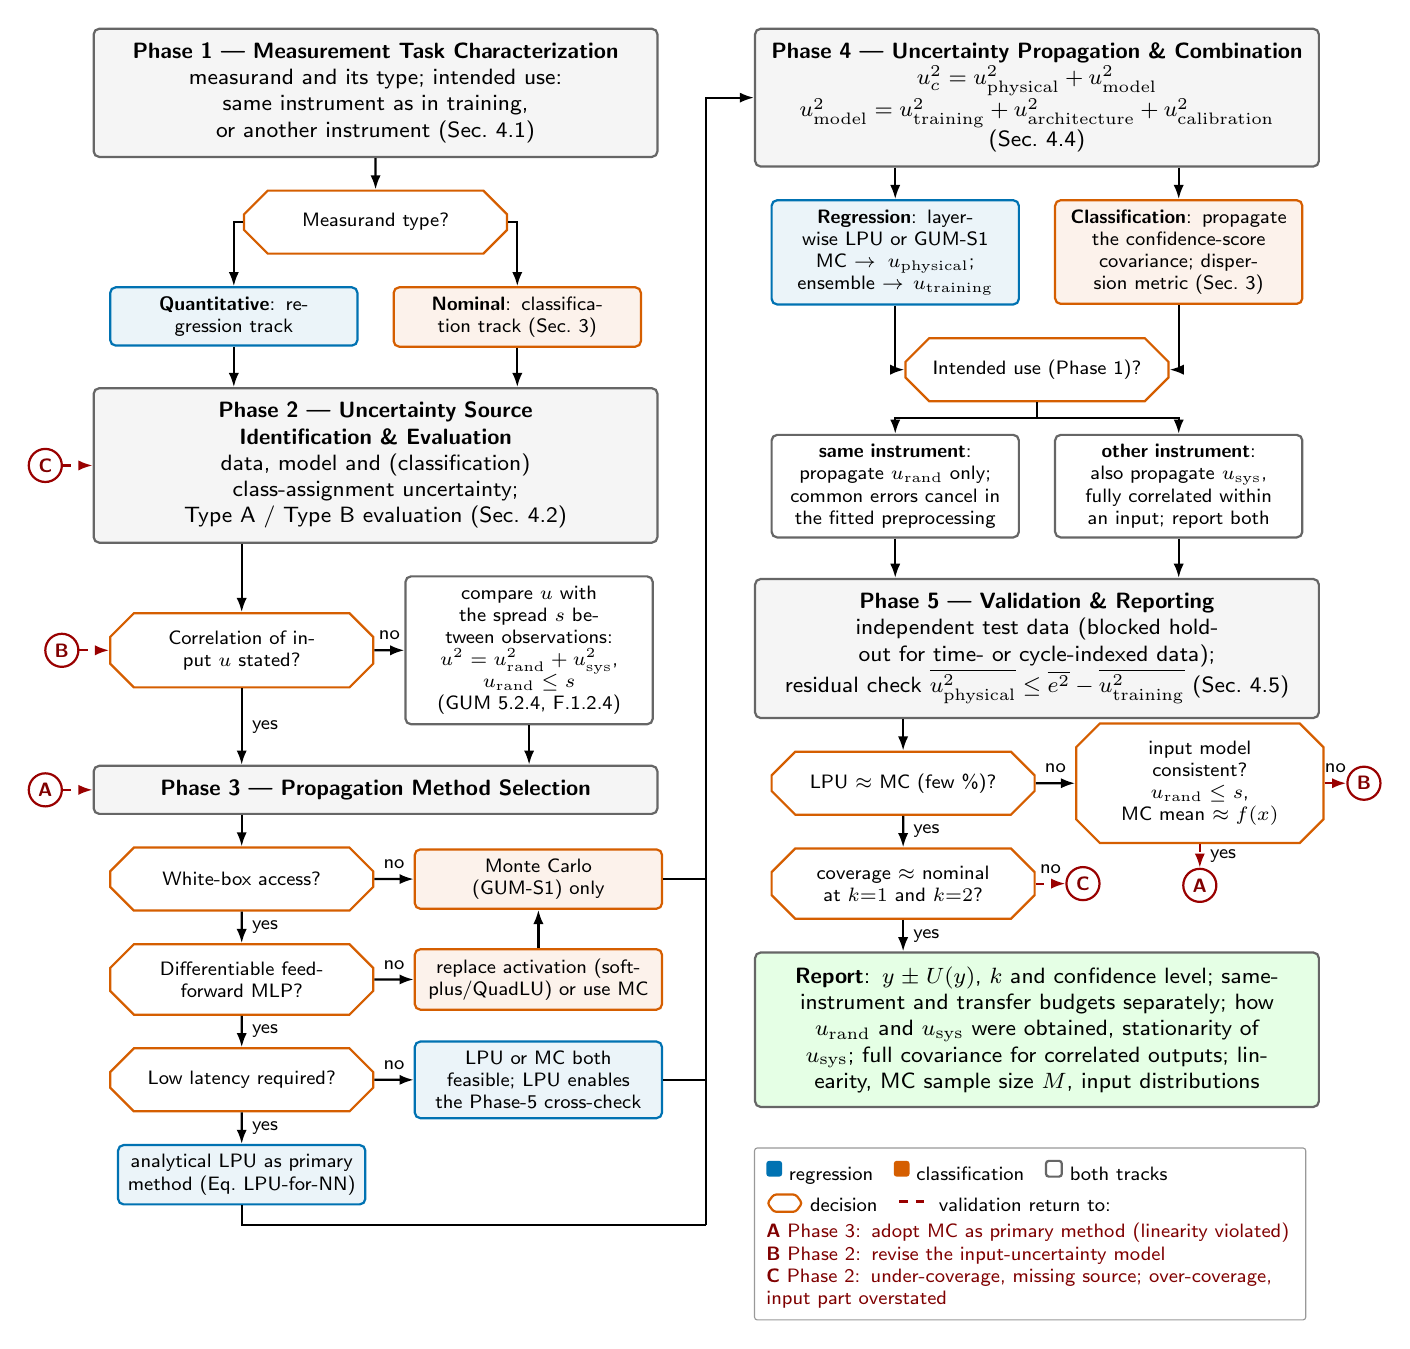
\begin{tikzpicture}[
  font=\sffamily\scriptsize,
  phase/.style={rectangle, rounded corners=2pt, draw=black!60, thick,
    fill=black!4, text width=68mm, align=center, inner sep=1.8mm, font=\sffamily\footnotesize},
  decision/.style={chamfered rectangle, chamfered rectangle xsep=2mm, draw=okOrange, thick,
    fill=white, text width=27mm, align=center, inner sep=1.2mm, minimum height=8mm},
  outcomeR/.style={rectangle, rounded corners=2pt, draw=okBlue, thick, fill=okBlue!8,
    text width=29mm, align=center, inner sep=1.2mm},
  outcomeC/.style={rectangle, rounded corners=2pt, draw=okOrange, thick, fill=okOrange!8,
    text width=29mm, align=center, inner sep=1.2mm},
  action/.style={rectangle, rounded corners=2pt, draw=black!60, thick, fill=white,
    text width=29mm, align=center, inner sep=1.2mm},
  report/.style={rectangle, rounded corners=2pt, draw=black!60, thick, fill=green!10,
    text width=68mm, align=center, inner sep=1.8mm, font=\sffamily\footnotesize},
  arrow/.style={-{Latex[length=1.8mm,width=1.3mm]}, thick},
  line/.style={thick},
  fbarrow/.style={-{Latex[length=1.8mm,width=1.3mm]}, thick, dashed, draw=red!60!black},
  conn/.style={circle, draw=red!60!black, thick, fill=white, text=red!50!black,
    font=\sffamily\scriptsize\bfseries, inner sep=0.4mm, minimum size=4.2mm},
  fblbl/.style={text=red!50!black, align=left, font=\sffamily\scriptsize},
  lbl/.style={font=\sffamily\scriptsize, midway}
]
% Column axes: left x = 0 (Phases 1-3), right x = 84 mm (Phases 4-5).
% Within a column, decisions sit 17 mm left of the axis and side outcomes
% 19 mm right of it; the gutter between the columns (x = 42 mm) carries the
% only connector from Phase 3 to Phase 4.
\coordinate (L) at (0,0);
\coordinate (R) at (84mm,0);
\coordinate (G) at (42mm,0);

% ================= LEFT COLUMN =================
% ---- Phase 1 ----
\node[phase, anchor=north] (p1) at (L) {\textbf{Phase 1 --- Measurement Task Characterization}\\
  measurand and its type; intended use:\\
  same instrument as in training, or another instrument (Sec.~4.1)};
\node[decision, anchor=north] (d1) at ($(p1.south)+(0,-4mm)$) {Measurand type?};
\draw[arrow] (p1) -- (d1);
\node[outcomeR, anchor=north] (r1) at ($(d1.south)+(-18mm,-4mm)$) {\textbf{Quantitative}: regression track};
\node[outcomeC, anchor=north] (c1) at ($(d1.south)+(18mm,-4mm)$) {\textbf{Nominal}: classification track (Sec.~3)};
\draw[arrow] (d1.west) -| (r1.north);
\draw[arrow] (d1.east) -| (c1.north);

% ---- Phase 2 ----
\node[phase, anchor=north] (p2) at ($(L |- c1.south)+(0,-5mm)$)
  {\textbf{Phase 2 --- Uncertainty Source Identification \& Evaluation}\\
  data, model and (classification) class-assignment uncertainty;\\
  Type A / Type B evaluation (Sec.~4.2)};
\draw[arrow] (r1.south) -- (r1.south |- p2.north);
\draw[arrow] (c1.south) -- (c1.south |- p2.north);
\node[action, anchor=north] (split) at ($(p2.south)+(19.5mm,-4mm)$)
  {compare $u$ with the spread $s$ between observations:\\
   \mbox{$u^2 = u_{\mathrm{rand}}^2 + u_{\mathrm{sys}}^2$,} \mbox{$u_{\mathrm{rand}} \le s$}\\
   (GUM 5.2.4, F.1.2.4)};
\coordinate (dcx) at ($(p2.south)+(-17mm,0)$);
\node[decision] (dcorr) at (dcx |- split.center) {Correlation of input $u$ stated?};
\draw[arrow] (dcorr.north |- p2.south) -- (dcorr.north);
\draw[arrow] (dcorr) -- (split) node[lbl, above]{no};

% ---- Phase 3 ----
\node[phase, anchor=north] (p3) at ($(L |- split.south)+(0,-5mm)$)
  {\textbf{Phase 3 --- Propagation Method Selection}};
\draw[arrow] (dcorr.south) -- (dcorr.south |- p3.north) node[lbl, right]{yes};
\draw[arrow] (split.south) -- (split.south |- p3.north);
\node[decision, anchor=north] (d2) at ($(p3.south)+(-17mm,-4mm)$) {White-box access?};
\draw[arrow] (d2.north |- p3.south) -- (d2.north);
\node[outcomeC, anchor=west] (mcOnly) at ($(d2.east)+(5mm,0)$) {Monte Carlo (GUM-S1) only};
\draw[arrow] (d2) -- (mcOnly) node[lbl, above]{no};
\node[decision, anchor=north] (d3) at ($(d2.south)+(0,-4mm)$) {Differentiable feed-forward MLP?};
\draw[arrow] (d2) -- (d3) node[lbl, right]{yes};
\node[outcomeC, anchor=west] (fixAct) at (mcOnly.west |- d3) {replace activation (softplus/QuadLU) or use MC};
\draw[arrow] (d3) -- (fixAct) node[lbl, above]{no};
\draw[arrow] (fixAct) -- (mcOnly);
\node[decision, anchor=north] (d4) at ($(d3.south)+(0,-4mm)$) {Low latency required?};
\draw[arrow] (d3) -- (d4) node[lbl, right]{yes};
\node[outcomeR, anchor=west] (lpuOrMc) at (mcOnly.west |- d4) {LPU or MC both feasible; LPU enables the Phase-5 cross-check};
\draw[arrow] (d4) -- (lpuOrMc) node[lbl, above]{no};
\node[outcomeR, anchor=north] (lpuPrimary) at ($(d4.south)+(0,-4mm)$) {analytical LPU as primary method (Eq.~LPU-for-NN)};
\draw[arrow] (d4) -- (lpuPrimary) node[lbl, right]{yes};

% ---- Phase 3 -> Phase 4 through the gutter ----
\draw[line] (mcOnly.east) -- (G |- mcOnly.east);
\draw[line] (lpuOrMc.east) -- (G |- lpuOrMc.east);
\draw[line] (lpuPrimary.south) -- ++(0,-2.5mm) coordinate (lpBase) -- (G |- lpBase);

% ================= RIGHT COLUMN =================
% ---- Phase 4 ----
\node[phase, anchor=north] (p4) at (R)
  {\textbf{Phase 4 --- Uncertainty Propagation \& Combination}\\
  \mbox{$u_c^2 = u_{\mathrm{physical}}^2 + u_{\mathrm{model}}^2$}\\
  \mbox{$u_{\mathrm{model}}^2 = u_{\mathrm{training}}^2 + u_{\mathrm{architecture}}^2 + u_{\mathrm{calibration}}^2$}\\
  (Sec.~4.4)};
\draw[arrow] (G |- lpBase) -- (G |- p4.west) -- (p4.west);
\node[outcomeR, anchor=north] (p4r) at ($(p4.south)+(-18mm,-4mm)$)
  {\textbf{Regression}: layer-wise LPU or GUM-S1 MC $\rightarrow u_{\mathrm{physical}}$; ensemble $\rightarrow u_{\mathrm{training}}$};
\node[outcomeC, anchor=north] (p4c) at ($(p4.south)+(18mm,-4mm)$)
  {\textbf{Classification}: propagate the confidence-score covariance; dispersion metric (Sec.~3)};
\draw[arrow] (p4r.north |- p4.south) -- (p4r.north);
\draw[arrow] (p4c.north |- p4.south) -- (p4c.north);
\node[decision, anchor=north] (duse) at ($(R |- p4r.south)+(0,-4mm)$) {Intended use (Phase 1)?};
\draw[arrow] (p4r.south) |- (duse.west);
\draw[arrow] (p4c.south) |- (duse.east);
\node[action, anchor=north] (same) at ($(duse.south)+(-18mm,-4mm)$)
  {\textbf{same instrument}: propagate $u_{\mathrm{rand}}$ only; common errors cancel in the fitted preprocessing};
\node[action, anchor=north] (transfer) at ($(duse.south)+(18mm,-4mm)$)
  {\textbf{other instrument}: also propagate $u_{\mathrm{sys}}$, fully correlated within an input; report both};
\draw[arrow] (duse.south) -- ++(0,-2mm) -| (same.north);
\draw[arrow] (duse.south) -- ++(0,-2mm) -| (transfer.north);

% ---- Phase 5 ----
\node[phase, anchor=north] (p5) at ($(R |- same.south)+(0,-5mm)$)
  {\textbf{Phase 5 --- Validation \& Reporting}\\
  independent test data (blocked hold-out for time- or cycle-indexed data);\\
  residual check \mbox{$\overline{u_{\mathrm{physical}}^2} \le \overline{e^2} - \overline{u_{\mathrm{training}}^2}$} (Sec.~4.5)};
\draw[arrow] (same.south) -- (same.south |- p5.north);
\draw[arrow] (transfer.south) -- (transfer.south |- p5.north);
\node[decision, anchor=north] (d5) at ($(p5.south)+(-17mm,-4mm)$) {LPU $\approx$ MC (few \%)?};
\draw[arrow] (d5.north |- p5.south) -- (d5.north);
\node[decision, anchor=west, text width=25mm] (d5b) at ($(d5.east)+(5mm,0)$)
  {input model consistent?\\ \mbox{$u_{\mathrm{rand}} \le s$,} \mbox{MC mean $\approx f(x)$}};
\draw[arrow] (d5) -- (d5b) node[lbl, above]{no};
\node[decision, anchor=north] (d6) at ($(d5.south)+(0,-4mm)$) {coverage $\approx$ nominal at $k{=}1$ and $k{=}2$?};
\draw[arrow] (d5) -- (d6) node[lbl, right]{yes};
\node[report, anchor=north] (rep) at ($(R |- d6.south)+(0,-4mm)$)
  {\textbf{Report}: $y \pm U(y)$, $k$ and confidence level; same-instrument and
  transfer budgets separately; how $u_{\mathrm{rand}}$ and $u_{\mathrm{sys}}$ were obtained,
  stationarity of $u_{\mathrm{sys}}$; full covariance for correlated outputs;
  linearity, MC sample size $M$, input distributions};
\draw[arrow] (d6.south) -- (d6.south |- rep.north) node[lbl, right]{yes};

% ---- validation returns: lettered connectors ----
% sources (Phase 5)
\node[conn, anchor=north] (A1) at ($(d5b.south)+(0,-3mm)$) {A};
\draw[fbarrow] (d5b.south) -- (A1) node[lbl, right]{yes};
\node[conn] (B1) at ($(d5b.east)+(5mm,0)$) {B};
\draw[fbarrow] (d5b.east) -- (B1) node[lbl, above]{no};
\node[conn] (C1) at ($(d6.east)+(6mm,0)$) {C};
\draw[fbarrow] (d6.east) -- (C1) node[lbl, above]{no};
% targets (left column, west side)
\node[conn] (A2) at ($(p3.west)+(-6mm,0)$) {A};
\draw[fbarrow] (A2) -- (p3.west);
\node[conn] (B2) at ($(dcorr.west)+(-6mm,0)$) {B};
\draw[fbarrow] (B2) -- (dcorr.west);
\node[conn] (C2) at ($(p2.west)+(-6mm,0)$) {C};
\draw[fbarrow] (C2) -- (p2.west);

% ---- legend and connector key (below the Report box) ----
\node[draw=black!40, fill=white, rounded corners=1pt, font=\sffamily\scriptsize, align=left,
      anchor=north west, inner sep=1.5mm, text width=67mm] (legend) at ($(rep.south west)+(0,-5mm)$) {
  \tikz[baseline=-0.5mm]\fill[okBlue] (0,0) rectangle (2mm,2mm); regression\quad
  \tikz[baseline=-0.5mm]\fill[okOrange] (0,0) rectangle (2mm,2mm); classification\quad
  \tikz[baseline=-0.5mm]\draw[black!60,thick] (0,0) rectangle (2mm,2mm); both tracks\\[0.8mm]
  \tikz[baseline=-0.2mm]\draw[okOrange,thick] (0,0.9mm)--(0.8mm,2mm)--(3.6mm,2mm)--(4.4mm,0.9mm)--(3.6mm,-0.2mm)--(0.8mm,-0.2mm)--cycle; decision\quad
  \tikz[baseline=-0.5mm]\draw[red!60!black,thick,dashed] (0,0.8mm) -- (4mm,0.8mm); validation return to:\\[0.5mm]
  {\color{red!50!black}\textbf{A} Phase 3: adopt MC as primary method (linearity violated)\\
  \textbf{B} Phase 2: revise the input-uncertainty model\\
  \textbf{C} Phase 2: under-coverage, missing source; over-coverage, input part overstated}
};

\end{tikzpicture}%
\end{lrbox}%
% crop the page to the picture
\pdfpagewidth=\dimexpr\wd\figbox+2\figborder\relax
\pdfpageheight=\dimexpr\ht\figbox+\dp\figbox+2\figborder\relax
\pdfhorigin=\figborder
\pdfvorigin=\figborder
\shipout\hbox{\usebox{\figbox}}
\end{document}
